\section{}

\textbf{Tiempo de lectura:} \{s15-reading-time\}

La memoria es un recurso central para el funcionamiento de un sistema
operativo moderno, puesto que es el único medio de almacenamiento al que
la CPU puede acceder directamente. Por ello, para que un programa pueda
ser ejecutado, debe ser cargado en la memoria desde el disco y creadas o
modificadas las estructuras internas del sistema operativo necesarias
para convertirlo en un proceso. Además, dependiendo de la forma en la
que se gestiona la memoria, los procesos ---o partes de los mismos---
pueden moverse de la memoria al disco ---y viceversa--- durante su
ejecución, con el objetivo de ajustar las necesidades de memoria para
mantener el \textbf{uso de la CPU} lo más alto posible.

Como comentamos en el \hyperref[_sistemas_multiprogramados]{???}, en los
\textbf{sistemas multiprogramados} existe una \textbf{cola de entrada},
que se define como aquella formada por el conjunto de procesos en disco
que esperan para ser cargados en la memoria para su ejecución.

Por tanto, el procedimiento normal de ejecución de un programa en dichos
sistemas es:

\begin{enumerate}
\def\labelenumi{\arabic{enumi}.}
\item
  Seleccionar un proceso de la cola de entrada y cargarlo en la memoria.
\item
  Mientras el proceso se ejecuta, este accede a instrucciones y datos de
  la memoria.
\item
  Finalmente, el proceso termina y su espacio en memoria es marcado como
  disponible.
\end{enumerate}

En los sistemas de propósito general modernos ---desde los
\textbf{sistemas de tiempo compartido} y los primeros \textbf{sistemas
de escritorio}--- no existe \textbf{cola de entrada}, por lo que los
programas se cargan inmediatamente en memoria cuando los usuarios
solicitan su ejecución. Excepto por eso, el procedimiento normal de
ejecución de un programa es similar al de los \textbf{sistemas
multiprogramados}.

\section{Etapas de un programa de
usuario}\label{_etapas_de_un_programa_de_usuario}

En la mayor parte de los casos, un programa de usuario debe pasar por
diferentes etapas ---algunas de las cuales son opcionales--- antes de
ser ejecutado (véase la
\hyperref[fig-etapas-programas-de-usuario]{Etapas de procesamiento de un
programa de usuario.}).

\begin{figure}
\centering
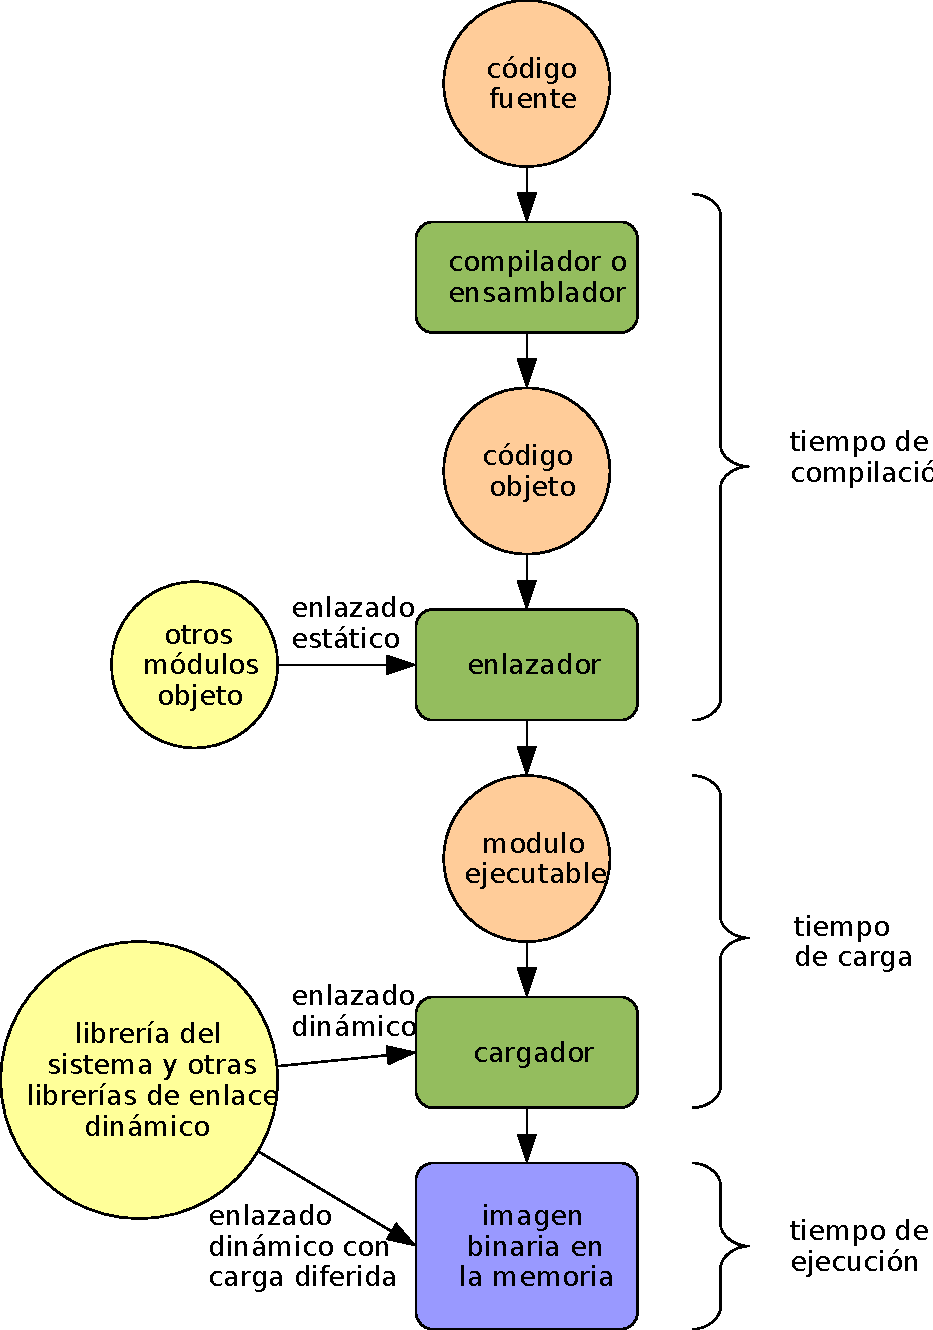
\includegraphics[width=0.8\textwidth]{media/C15_memoria_principal/etapas_de_un_programa_de_usuario.pdf}
\caption{Etapas de procesamiento de un programa de
usuario.}\label{fig-etapas-programas-de-usuario}
\end{figure}

Los archivos de \textbf{código fuente}{} del programa son compilados por
el compilador, generando un archivo de
\href{https://es.wikipedia.org/wiki/C\%C3\%B3digo_objeto}{\textbf{código
objeto}} ---con extensiones \texttt{.o} u \texttt{.obj}--- para cada
uno.

Todos los archivos de \textbf{código objeto}{} son unidos por el
enlazador para crear el archivo \textbf{ejecutable}, en una fase que se
denomina \textbf{enlazado estático}{}. En esta fase también se pueden
incorporar al ejecutable \textbf{librerías de enlace estático}{} ---con
extensiones \texttt{.a} o \texttt{.lib}--- con \textbf{código objeto}
que ha sido empaquetado para ser reutilizado en múltiples ejecutables.

El compilador y el enlazador suelen ser dos programas independientes,
aunque en ocasiones el compilador se haga cargo de ambas fases por
comodidad. Por ejemplo, en los sistemas GNU el compilador \{cmd\_gcc\}
por defecto genera el \textbf{código objeto} en archivos temporales,
luego invoca al enlazador \{cmd\_ld\} para crear el \textbf{ejecutable}
y finalmente elimina los archivos temporales.

En proyectos grandes suele ser más interesante usar ambas herramientas
por separado para reducir el tiempo de compilación. El compilador genera
los archivos de \textbf{código objeto}, que se conservan entre
compilaciones. Así, cada vez que se quiere generar una nueva versión del
ejecutable, solo es necesario compilar los archivos de \textbf{código
fuente} que hayan cambiado y luego enlazar juntos todos los archivos de
\textbf{código objeto}.

Al crear el \textbf{ejecutable} se pueden guardar en él dependencias
respecto a librerías que se enlazarán posteriormente, durante la carga o
ejecución del programa, en una fase denominada \textbf{enlazado
dinámico}{}.

En el momento en el que se va a ejecutar el programa, cuando está
construyendo la imagen binaria del proceso en la memoria; el sistema
operativo examina estas dependencias, carga las \textbf{librerías de
enlace dinámico}{} indicadas ---con extensiones \texttt{.so},
\texttt{dylib} o \texttt{.dll}--- y resuelve las referencias del
programa sus variables y funciones. Las \textbf{librerías de enlace
dinámico} contienen \textbf{código objeto}, enlazado en un formato
especial de \textbf{ejecutable} diseñado para contener partes
compartidas entre archivos ejecutables.

Este proceso puede ocurrir mientras se carga el \textbf{ejecutable}
---como se ha descrito--- o cuando el programa usa por primera vez un
elemento de las \textbf{librerías de enlace dinámico}. También es común
que el sistema ofrezca funciones para que los programas puedan cargar
manualmente e invocar funciones de \textbf{librerías de enlace
dinámico}. Esto es muy útil para crear programas que se puedan mejorar
por medio de extensiones o \emph{plugins}.

\begin{longtable}[]{@{}
  >{\raggedright\arraybackslash}p{(\linewidth - 6\tabcolsep) * \real{0.2500}}
  >{\raggedright\arraybackslash}p{(\linewidth - 6\tabcolsep) * \real{0.2500}}
  >{\raggedright\arraybackslash}p{(\linewidth - 6\tabcolsep) * \real{0.2500}}
  >{\raggedright\arraybackslash}p{(\linewidth - 6\tabcolsep) * \real{0.2500}}@{}}
\caption{Extensiones de archivos de programas.}\tabularnewline
\toprule\noalign{}
\begin{minipage}[b]{\linewidth}\raggedright
\end{minipage} & \begin{minipage}[b]{\linewidth}\raggedright
UNIX, Linux y otros sistemas estilo UNIX
\end{minipage} & \begin{minipage}[b]{\linewidth}\raggedright
macOS
\end{minipage} & \begin{minipage}[b]{\linewidth}\raggedright
Microsoft Windows
\end{minipage} \\
\midrule\noalign{}
\endfirsthead
\toprule\noalign{}
\begin{minipage}[b]{\linewidth}\raggedright
\end{minipage} & \begin{minipage}[b]{\linewidth}\raggedright
UNIX, Linux y otros sistemas estilo UNIX
\end{minipage} & \begin{minipage}[b]{\linewidth}\raggedright
macOS
\end{minipage} & \begin{minipage}[b]{\linewidth}\raggedright
Microsoft Windows
\end{minipage} \\
\midrule\noalign{}
\endhead
\bottomrule\noalign{}
\endlastfoot
\textbf{Código objeto} & \texttt{.o} & \texttt{.o} & \texttt{.obj} \\
\textbf{Librería de enlace estático} & \texttt{.a} & \texttt{.a} &
\texttt{.lib} \\
\textbf{Ejecutable} & & & \texttt{.exe} \\
\textbf{Librería de enlace dinámico} & \texttt{.so} & \texttt{.so},
\texttt{.dylib} & \texttt{.dll} \\
\textbf{Formato de ejecutables y librerías de enlace dinámico} &
\href{https://es.wikipedia.org/wiki/Executable_and_Linkable_Format}{Executable
and Linkable Format} (ELF) &
\href{https://en.wikipedia.org/wiki/Mach-O}{Mach-O} &
\href{https://es.wikipedia.org/wiki/Portable_Executable}{Portable
Executable} (PE) \\
\end{longtable}

\section{Reubicación de las
direcciones}\label{_reubicaciuxf3n_de_las_direcciones}

La mayor parte de los sistemas permiten que un proceso de usuario resida
en cualquier parte de la memoria física. Así, aunque el espacio de
direcciones del sistema comience en \texttt{0x00000000}, la primera
dirección del proceso de usuario no tiene por qué ser esa.

En cada una de las etapas vistas en el
\hyperref[_etapas_de_un_programa_de_usuario]{Etapas de un programa de
usuario} las direcciones pueden representarse de formas distintas, por
lo que en cada paso es necesario reasignar las direcciones usadas en una
etapa en direcciones de la siguiente.

Por ejemplo, en el código fuente de un programa las direcciones son
generalmente simbólicas, como los nombres de las variables y las
funciones. A continuación, un compilador suele reasignar esas
direcciones simbólicas en \textbf{direcciones reubicables}{} del estilo
de «120 bytes desde el comienzo del módulo». Finalmente ---el
enlazador--- que genera el ejecutable--- o el cargador ---que carga el
programa en la memoria--- convierte esas \textbf{direcciones
reubicables} en \textbf{direcciones absolutas}{}, como
\texttt{0x00210243}.

Por tanto, en cada etapa se traducen las direcciones de un espacio de
direcciones en el siguiente. Sin embargo, para que al final el programa
pueda ser ejecutado, es necesario que tanto a los datos como a las
instrucciones se les reasignen en algún momento a \textbf{direcciones
absolutas} de la memoria. Esto puede ocurrir en \textbf{tiempo de
compilación}, \textbf{tiempo de carga} o \textbf{tiempo de ejecución}

\subsection{Reubicación en tiempo de
compilación}\label{_reubicaciuxf3n_en_tiempo_de_compilaciuxf3n}

Si durante la compilación o el enlazado se conoce el lugar de la memoria
donde va a ser ejecutado el proceso, se puede generar directamente
código con \textbf{direcciones absolutas} o \textbf{código absoluto}{}.

Eso significa que si en algún momento la dirección de inicio donde es
cargado el programa cambia, es necesario recompilar el código fuente del
programa para poder ejecutarlo en la nueva ubicación.

Un ejemplo son los ejecutables con formato
\href{https://es.wikipedia.org/wiki/Archivo_COM}{COM} del sistema
operativo MS-DOS. Estos ejecutables no eran reubicables, aunque podían
ponerse en distintas ubicaciones de la memoria gracias a la
\href{https://es.wikipedia.org/wiki/Segmentaci\%C3\%B3n_de_memoria_del_x86}{segmentación
de memoria de la familia Intel x86}.

\subsection{Reubicación en tiempo de
carga}\label{_reubicaciuxf3n_en_tiempo_de_carga}

Si no se conoce durante la compilación el lugar donde va a residir un
programa cuando sea ejecutado, el compilador y el enlazador deben
generar ejecutables con \textbf{código reubicable}{}.

En este tipo de código se utilizan \textbf{direcciones reubicables}, de
manera que se retrasa su asignación a \textbf{direcciones absolutas}
hasta el momento de la carga del programa. Esto permite que un programa
pueda residir en cualquier parte de la memoria física, cargando los
procesos donde más convenga para maximizar el aprovechamiento de la
misma.

Para generar \textbf{código reubicable}, por lo general, el compilador
genera \textbf{código independiente de la posición}{} o \textbf{{}PIC}
(\emph{Position-Independent Code}). Este tipo de código se puede
ejecutar adecuadamente y sin modificaciones independientemente del lugar
de la memoria donde esté ubicado, porque utiliza direcciones relativas.

Lamentablemente, esto puede limitar las características de la CPU que
puede utilizar el compilador o, a veces, las instrucciones que usan
direcciones absolutas son más rápidas que las que usan direcciones
relativas, aunque en los procesadores modernos la diferencia apenas es
perceptible.

Por ejemplo, las CPU x86-64 soportan un modo de direccionamiento en el
que las direcciones son relativas a la dirección en el contador de
programa. Esto simplifica generar código reubicable eficiente. Sin
embargo, en las CPU x86 anteriores, las instrucciones de salto podían
ser relativas al contador de programa, pero no ocurría así con aquellas
destinadas a acceder a los datos del programa.

Cuando no se puede o no es eficiente generar \textbf{código
independiente de la posición} se puede recurrir al uso de \textbf{tablas
de reubicación} en tiempo de carga. En este caso el compilador y el
enlazador generan:

\begin{enumerate}
\def\labelenumi{\arabic{enumi}.}
\item
  Código con direcciones relativas a cierta dirección fija del
  ejecutable ---como el comienzo de la sección de código--- o
  direcciones absolutas calculadas bajo la suposición de que el
  ejecutable se va a poder cargar en cierta dirección concreta de la
  memoria, que suele guardarse en la cabecera del ejecutable.
\item
  Una \textbf{tabla de reubicaciones}{} que se almacena en el mismo
  ejecutable. Esta tabla contiene punteros a las ubicaciones en el
  código del ejecutable de las direcciones que deben reubicarse al
  cargarlo.
\end{enumerate}

Durante la carga, el cargador del sistema operativo, una vez ha copiado
a la memoria el contenido del ejecutable y conoce la ubicación
definitiva del programa, recorre la \textbf{tabla de reubicaciones} para
buscar las \textbf{direcciones reubicables} y actualizarlas.

Supongamos que en un sistema Linux x86-64 tenemos el siguiente código en
un archivo de nombre \texttt{test.c}:

\begin{Shaded}
\begin{Highlighting}[]
\DataTypeTok{long}\NormalTok{ i }\OperatorTok{=} \DecValTok{10}\OperatorTok{;}

\DataTypeTok{int}\NormalTok{ test}\OperatorTok{()}
\OperatorTok{\{}
\NormalTok{    i }\OperatorTok{=} \DecValTok{12}\OperatorTok{;}
    \ControlFlowTok{return} \DecValTok{0}\OperatorTok{;}
\OperatorTok{\}}

\DataTypeTok{int}\NormalTok{ main}\OperatorTok{()}
\OperatorTok{\{}
\NormalTok{    i }\OperatorTok{=} \DecValTok{11}\OperatorTok{;}
    \ControlFlowTok{return}\NormalTok{ test}\OperatorTok{();}
\OperatorTok{\}}
\end{Highlighting}
\end{Shaded}

En lugar de compilarlo para generar el ejecutable final, podemos usar la
opción \texttt{-c} del compilador \{cmd\_gcc\} para que solo genere el
archivo de \textbf{código objeto} correspondiente. Después podemos usar
el comando \{cmd\_objdump\} para examinar el \textbf{código objeto}:

\begin{verbatim}
$ gcc -c test.c
$ objdump -d test.o

test.o:     file format elf64-x86-64


Disassembly of section .text:

0000000000000000 <test>:                                
   0:   f3 0f 1e fa             endbr64
   4:   55                      push   %rbp
   5:   48 89 e5                mov    %rsp,%rbp
   8:   48 c7 05 00 00 00 00    movq   $0xc,0x0(%rip)   
   f:   0c 00 00 00
  13:   b8 00 00 00 00          mov    $0x0,%eax
  18:   5d                      pop    %rbp
  19:   c3                      retq

000000000000001a <main>:                                
  1a:   f3 0f 1e fa             endbr64
  1e:   55                      push   %rbp
  1f:   48 89 e5                mov    %rsp,%rbp
  22:   48 c7 05 00 00 00 00    movq   $0xb,0x0(%rip)   
  29:   0b 00 00 00
  2d:   b8 00 00 00 00          mov    $0x0,%eax
  32:   e8 00 00 00 00          callq  37 <main+0x1d>   
  37:   5d                      pop    %rbp
  38:   c3                      retq
\end{verbatim}

\begin{itemize}
\item
  El archivo de \textbf{código objeto} se divide en varias secciones o
  segmentos. En el \textbf{segmento de código}{} o \textbf{.text}{} se
  almacenan las funciones compiladas del código original. Cada función
  tiene una ubicación, que es relativa a su posición dentro del segmento
  de código en el archivo.

  Obviamente, estas no son las direcciones definitivas en las que se
  ejecutarán estas funciones cuando el ejecutable sea cargado en la
  memoria, por lo que este \textbf{código objeto} generado por el
  compilador debe ser \textbf{código reubicable}.
\item
  \texttt{callq} es la instrucción encargada de invocar a
  \texttt{test()} desde \texttt{main()}, pero si ejecutamos este código
  en su estado actual, la ejecución saltaría a la instrucción en 0x37,
  es decir, a la siguiente tras \texttt{callq}. Esto no es un error del
  compilador, sino que el compilador no ha puesto la dirección correcta
  porque aún desconoce cuál será la ubicación definitiva de
  \texttt{test()}.

  En x86-64 las instrucciones de salto como \texttt{callq} hacen saltos
  relativos al contador de programa ---almacenado en un registro
  llamando \texttt{rip}---. Todas estas instrucciones llevan un
  desplazamiento que se suma al valor actual de \texttt{rip}, que
  contiene la dirección en la memoria de la siguiente instrucción. Como
  el compilador no sabe donde estará \texttt{test()}, deja este
  desplazamiento a 0 ---por eso los bytes \textquotesingle00 00 00
  00\textquotesingle{} en la codificación de la instrucción
  \texttt{callq}--- por lo que el salto será a la siguiente instrucción.
\item
  En el acceso a la variable \texttt{i} para cambiar su valor, ocurre
  algo parecido. La dirección se escribe relativa al contador de
  programa \texttt{rip}, pero como el compilador no sabe la posición
  definitiva de la variable, deja el desplazamiento a 0. Por eso el
  desensamblado indica lo de \texttt{0x0(\%rip)}, que quiere decir:
  dirección desplazada 0 respecto a \texttt{rip}.
\end{itemize}

Durante el enlazado, para generar el ejecutable definitivo, es necesario
saber dónde están en el código las direcciones que se deben reubicar.
Para eso el archivo de \textbf{código objeto} lleva una \textbf{tabla de
reubicación}, que también se puede leer con \{cmd\_objdump\}:

\begin{verbatim}
$ objdump -r test.o
test.o:     file format elf64-x86-64

RELOCATION RECORDS FOR [.text]:
OFFSET           TYPE              VALUE
000000000000000b R_X86_64_PC32     i-0x0000000000000008
0000000000000025 R_X86_64_PC32     i-0x0000000000000008
0000000000000033 R_X86_64_PLT32    test-0x0000000000000004
\end{verbatim}

En nuestro ejemplo la tabla contiene tres entradas, dos para las dos
instrucciones que modifican la variable \texttt{i} y una para la
instrucción \texttt{callq} que sirve para invocar \texttt{test()}. La
primera columna indica la ubicación en \textbf{.text} de la dirección
que se debe reubicar. Mientras la segunda columna especifica el tipo de
reubicación y la tercera contiene información adicional que hace falta
para realizar la reubicación.

Por ejemplo, la primera entrada del ejemplo indica que debe desplazarse
en \texttt{0x08} la dirección a reubicar en \texttt{0x0b} ---el acceso a
\texttt{i} en \texttt{test()} para que apunte a la dirección de la
variable \texttt{i}.

\subsection{Reubicación en tiempo de
ejecución}\label{_reubicaciuxf3n_en_tiempo_de_ejecuciuxf3n}

Si un proceso puede ser movido durante su ejecución de un lugar de la
memoria a otro, la reubicación de direcciones debe ser retrasada hasta
el momento de la ejecución de cada instrucción del programa.

Para que esto sea posible, necesitamos disponer de hardware especial que
suele estar presente en la mayor parte de las CPU modernas, por lo que
la inmensa mayoría de los sistemas operativos de propósito general
modernos utilizan este método. De él hablaremos en el
\hyperref[_espacio_de_direcciones_virtual_frente_a_fuxedsico]{Espacio de
direcciones virtual frente a físico}.

\section{Espacio de direcciones virtual frente a
físico}\label{_espacio_de_direcciones_virtual_frente_a_fuxedsico}

En el \hyperref[_protecciuxf3n_de_la_memoria]{???} vimos en los sistemas
operativos modernos, como medida de protección, los procesos no tienen
acceso libre a la memoria física.

\begin{figure}
\centering
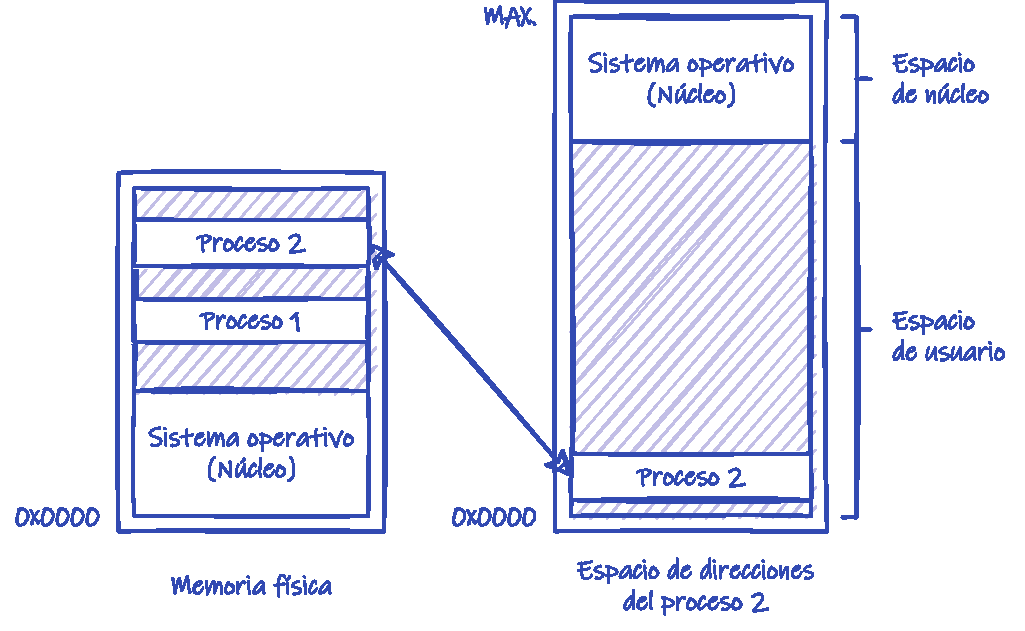
\includegraphics[width=0.8\textwidth]{media/C15_memoria_principal/protección_memoria.pdf}
\caption{Mapeo de la memoria física en el espacio de direcciones virtual
de un proceso.}\label{fig-espacio-direcciones-virtual-frente-fuxedsico}
\end{figure}

En lugar de eso el sistema operativo ---asistido por la \textbf{{}MMU}
(\emph{Memory-Management Unit})--- proporciona a cada proceso un
\textbf{espacio de direcciones virtual}{} que ofrece una «vista» privada
de la memoria, similar a la que tendrían si cada uno de los procesos
estuviera siendo ejecutando en solitario (véase la
\hyperref[fig-espacio-direcciones-virtual-frente-fuxedsico]{Mapeo de la
memoria física en el espacio de direcciones virtual de un proceso.}). Es
durante los accesos a la memoria principal en tiempo de ejecución,
cuando estas \textbf{direcciones virtuales}{} son convertidas por la
\textbf{MMU} en las \textbf{direcciones físicas}{}, con las que
realmente se accede a la memoria. El \textbf{espacio de direcciones
físico}{} es el conjunto de direcciones físicas que corresponden a todas
las direcciones virtuales de un \textbf{espacio de direcciones virtual}
dado.

El mecanismo de protección descrito es una forma muy común de
\textbf{reubicación de las direcciones en tiempo de ejecución}, que está
presente en la mayor parte de los sistemas operativos de propósito
general modernos. Pero, aparte de la protección de la memoria, algunas
otras características de dicho mecanismo son:

\begin{itemize}
\item
  Los procesos pueden ser cargados en cualquier zona libre de la memoria
  física e incluso movidos de una región a otra durante la ejecución de
  los procesos, puesto que la transformación de las \textbf{direcciones
  virtuales} en \textbf{direcciones físicas} se realiza durante la
  ejecución de cada instrucción.
\item
  El código generado por el compilador puede ser \textbf{código
  absoluto}, puesto que de antemano se sabe que todas las ubicaciones
  del espacio de direcciones virtual van a estar disponibles.

  Lo común es que los programas se ubiquen en una dirección fija en la
  parte baja del espacio de direcciones virtual. Por ejemplo, empezando
  en la dirección \texttt{0x00400000}, dejando libres los primeros 4 MiB
  del \textbf{espacio de direcciones virtual}.
\end{itemize}

Los programas pueden ubicarse en cualquier lugar del \textbf{espacio de
direcciones virtual}, pero no ocurre lo mismo con las \textbf{librerías
de enlace dinámico}, cuya posible ubicación va a depender del espacio
ocupado por el programa y por otras \textbf{librerías de enlace
dinámico}. Por tanto, como veremos en detalle más adelante, estas
librerías deben ser reubicables en tiempo de carga.

\begin{itemize}
\item
  Se puede reducir el consumo de memoria principal compartiendo las
  regiones de memoria física asignadas al código y los datos de solo
  lectura de los procesos de un mismo programa.
\end{itemize}

El código de un programa suele contener direcciones tanto para los
saltos como para el acceso a los datos. Al ubicar los programas en las
mismas regiones de los espacios de direcciones virtuales de sus
procesos, nos estamos asegurando de que el código en memoria de los
procesos de un mismo programa es el mismo ---pues todos usan las mismas
direcciones virtuales absolutas--- por lo que se puede compartir la
memoria física que ocupan.

En Linux cada proceso tiene su propio espacio de direcciones virtual,
por lo que los ejecutables pueden generarse para ser cargados en una
dirección fija, ya que es seguro que no habrá otro ocupando la misma
dirección.

Si la dirección donde se va a ejecutar el programa puede fijarse de
antemano, los ejecutables pueden contener \textbf{código absoluto}. Por
eso en Linux x86-64 el enlazador coge el \textbf{código objeto} que va a
formar parte del ejecutable, lo reubica asumiendo que el ejecutable se
cargará en cierta dirección de la memoria y genera un ejecutable con
\textbf{código absoluto}, sin \textbf{tablas de reubicación}.

Por ejemplo, si compilamos completamente el \texttt{test.c} anterior y
preguntamos por la \textbf{tabla de reubicación}, veremos que está
vacía:

\begin{verbatim}
$ gcc -o test test.c
$ objdump -r test
test.o:     file format elf64-x86-64
\end{verbatim}

Si desensamblamos el código, veremos que han cambiado algunas cosas en
\texttt{main()} y a \texttt{test()} respecto a lo que había en el
\textbf{código objeto}.

\begin{verbatim}
$ objdump -d test

test.o:     file format elf64-x86-64


Disassembly of section .text:

...

0000000000001129 <test>:                                           
    1129:       f3 0f 1e fa             endbr64
    112d:       55                      push   %rbp
    112e:       48 89 e5                mov    %rsp,%rbp
    1131:       c7 05 d9 2e 00 00 03    movl   $0x3,0x2ed9(%rip)   
    1138:       00 00 00
    113b:       b8 00 00 00 00          mov    $0x0,%eax
    1140:       5d                      pop    %rbp
    1141:       c3                      retq

0000000000001142 <main>:
    1142:       f3 0f 1e fa             endbr64
    1146:       55                      push   %rbp
    1147:       48 89 e5                mov    %rsp,%rbp
    114a:       c7 05 c0 2e 00 00 01    movl   $0x1,0x2ec0(%rip)   
    1151:       00 00 00
    1154:       b8 00 00 00 00          mov    $0x0,%eax
    1159:       e8 cb ff ff ff          callq  1129 <test>         
    115e:       5d                      pop    %rbp
    115f:       c3                      retq

...
\end{verbatim}

\begin{itemize}
\item
  Las instrucciones que acceden a la variable \texttt{i} ahora tienen el
  desplazamiento adecuado respecto al contador de programa \texttt{rip}
  para acceder a dicha variable.
\item
  La instrucción de salto tiene un desplazamiento que sumado al valor de
  \texttt{rip} lleva directamente al comienzo del código de la función
  \texttt{test()}.
\end{itemize}

\section{Enlazado dinámico y librerías
compartidas}\label{_enlazado_dinuxe1mico_y_libreruxedas_compartidas}

Como hemos comentado anteriormente, fundamentalmente existen dos tipos
de enlazado:

\begin{itemize}
\item
  En el \textbf{enlazado estático}{}, las librerías del sistema y otros
  módulos son combinados por el enlazador para formar la imagen binaria
  del programa que es almacenada en disco. Algunos sistemas operativos
  ---como MS-DOS--- solo soportan este tipo de enlazado.
\item
  En el \textbf{enlazado dinámico}{}, este se pospone hasta la carga o
  la ejecución\_ (véase la
  \hyperref[fig-etapas-programas-de-usuario]{Etapas de procesamiento de
  un programa de usuario.}).
\end{itemize}

Generalmente el enlazado dinámico ocurre durante la carga del programa:

\begin{enumerate}
\def\labelenumi{\arabic{enumi}.}
\item
  Durante la carga del ejecutable se comprueban las dependencias del
  mismo. Estas se almacenan en el mismo archivo en disco que dicho
  ejecutable.
\item
  Las librerías a enlazar se cargan y ubican en el espacio de
  direcciones virtual creado para el nuevo proceso.
\item
  Finalmente, las referencias del programa a las funciones de cada una
  de las librerías cargadas se actualizan con la dirección en memoria de
  las mismas. Así la invocación de las funciones por parte del programa
  se puede realizar de forma transparente, como si siempre hubieran
  formado parte del mismo.
\end{enumerate}

Cuando el enlazado se va a realizar en tiempo de ejecución se habla de
\textbf{enlazado dinámico con carga diferida}{}. En ese caso el
procedimiento es el siguiente:

\begin{enumerate}
\def\labelenumi{\arabic{enumi}.}
\item
  Durante el enlazado estático del ejecutable se pone un \emph{stub} a
  cada referencia a alguna función de la librería que va a ser enlazada
  dinámicamente.
\item
  Si durante la ejecución del programa alguna de dichas funciones es
  invocada, se ejecuta el \emph{stub}. El \emph{stub} es una pequeña
  pieza de código que sabe como cargar la librería, si no ha sido
  cargada previamente, y cómo localizar la función adecuada en la misma.
\item
  Finalmente, el \emph{stub} se sustituye a sí mismo con la dirección de
  la función y la invoca. Esto permite que la siguiente ejecución de la
  función no incurra en ningún coste adicional.
\end{enumerate}

Sin esta habilidad, cada programa en el sistema debería tener, por
ejemplo, una copia de la librería del sistema incluida en su ejecutable.
Esto significa un desperdicio de espacio libre en disco y de memoria
principal. Además, este esquema facilita la actualización de las
librerías, puesto que los programas pueden utilizar directamente las
versiones actualizadas sin necesidad de volver a ser enlazados.

\subsection{Reubicación de las
direcciones}\label{_reubicaciuxf3n_de_las_direcciones_2}

Durante la compilación de una \textbf{librería dinámica} no se conoce la
región que va a ocupar, dentro de los espacios de direcciones virtuales
de los distintos procesos que la van a utilizar, por lo que es necesario
generar \textbf{código reubicable}.

Atendiendo a lo visto en
\hyperref[_reubicaciuxf3n_en_tiempo_de_carga]{Reubicación en tiempo de
carga} existen fundamentalmente dos estrategias:

\begin{itemize}
\item
  El compilador puede generar \textbf{código independiente de la
  posición} (PIC). Esto permite reducir el consumo de memoria principal
  compartiendo las regiones de memoria física asignadas al código de una
  misma librería en los distintos procesos que la utilizan, pues en
  todas el código será exactamente el mismo.
\item
  En los sistemas operativos donde no se usa código PIC, el compilador
  debe generar código reubicable con \textbf{tablas de reubicación},
  para que la reubicación de las direcciones virtuales se haga en tiempo
  de carga. Esto aumenta el tiempo de carga de las librerías y solo
  permite que compartan memoria física partes de la librería que sigan
  siendo iguales tras la reubicación de las direcciones.
\end{itemize}

\subsection{Librerías compartidas}\label{_libreruxedas_compartidas}

{} Habitualmente las librerías incluyen información acerca de su
versión. Esta información puede ser utilizada para evitar que los
programas se ejecuten con versiones incompatibles de las mismas, o para
permitir que haya más de una versión de cada librería en el sistema. Así
los viejos programas se pueden ejecutar con las viejas versiones de las
librerías ---o con versiones actualizadas aunque compatibles--- mientras
los nuevos programas se ejecutan con las versiones más recientes e
incompatibles con los viejos programas.

A este sistema se lo conoce como \textbf{librerías compartidas}.

Para establecer correctamente la compatibilidad entre librerías y
programas, es conveniente y bastante común que los desarrolladores de
las \textbf{librerías compartidas} utilicen \textbf{versionado
semántico}. El \textbf{{}versionado semántico} es un convenio por el
cual el número de versión suele venir indicado por tres número separados
por puntos ---como, por ejemplo: 5.3.4--- de tal forma que:

\begin{itemize}
\item
  El primer número es incrementado cuando ocurre un cambio drástico en
  la librería, de tal forma que seguramente los programas hechos para
  versiones anteriores no van a ser compatibles con la nueva versión.
\item
  El segundo número es incrementado cuando se añade alguna nueva
  característica o se modifica alguna ya existente, pero el cambio no
  debe romper los programas hechos para la versión anterior.
\item
  El último número es incrementado al corregir errores, pero no se rompe
  la compatibilidad con versiones previas.
\end{itemize}

De esta forma, los desarrolladores pueden enlazar sus programas contra
la versión 5 de la librería, por ejemplo, sabiendo que así funcionarán
con cualquier versión actualizada o corregida ---como la 5.1, 5.2.9 o
5.10.1--- pero nunca podrán ejecutarse con versiones que tienen cambios
mayores y posiblemente incompatibles ---como la versión 6.1 o la
2.10---.

Volviendo al programa de ejemplo \texttt{test.c}, podemos obtener
fácilmente las librerías compartidas de las que depende usando el
comando \{cmd\_ldd\}:

\begin{verbatim}
$ ldd test
linux-vdso.so.1 (0x00007fffd833e000)
libc.so.6 => /lib/x86_64-linux-gnu/libc.so.6 (0x00007f47c20c9000)   
/lib64/ld-linux-x86-64.so.2 (0x00007f47c22cf000)                    
\end{verbatim}

\begin{itemize}
\item
  El ejecutable tiene que estar enlazado con la librería del sistema
  ---llamada \texttt{libc} en los sistemas POSIX--- para que pueda
  acceder a los servicios del sistema.

  \texttt{libc.so.6} es el nombre por el que se buscará el archivo que
  contiene la librería compartida de la librería del sistema Si se
  hubiera usado solamente \texttt{libc.so}, el ejecutable podría
  intentar usar cualquier versión de \texttt{libc}, pero al incluir el
  primer número de versión en el nombre, nos aseguramos de que el
  ejecutable solo usará versiones 6 de la librería del sistema. Así se
  evita ejecutar el programa con versiones que pueden ser incompatibles.
\item
  La librería \{linux\_ldso\} se encarga de las cuestiones relacionadas
  con el enlazado y carga dinámica de librerías.
\end{itemize}

Si estás librerías no estuvieran disponibles al intentar ejecutar el
programa, la ejecución fallaría, ya que son un requisito obligatorio.
Sin embargo, el enlazado dinámico no es algo que solo pueda configurarse
durante la compilación para que ocurra automáticamente durante la carga
del ejecutable. Los sistemas operativo modernos proporcionan funciones
para que un proceso pueda cargar cualquier y descargar librería durante
la ejecución y acceder a sus variables e invocar sus funciones. En los
sistemas POSIX estas funciones las proporciona la librería
\{linux\_ldso\}.

Esto es muy útil cuando se quiere que ciertas librerías sean opcionales.
Es decir, que no sea necesario tenerlas instaladas en el sistema donde
se va a ejecutar el programa, de tal forma que si no están disponibles,
el programa funcione con normalidad, pero si están instaladas, el
programa aproveche la funcionalidad adicional que proporcionan. Así es
como navegadores, editores y otros programas implementan extensiones y
\emph{plugins}, con los que el usuario puede extender la funcionalidad
del programa original sin recompilarlo. Estas extensiones generalmente
se implementan como librerías compartidas que el programa busca y carga
durante su ejecución.

Por lo general, la mayor parte de las librerías que usan los programas
son enlazadas dinámicamente, pero el enlazador siempre tiene que incluir
en el ejecutable algunas librerías enlazadas estáticamente que son
importantes para la ejecución del programa. Por eso al ejecutar
\texttt{objdump\ -d\ test} vemos funciones que no estaban ni en
\texttt{test.c\ ni\ en\ el\ archivo\ de\ código\ objeto\ \textasciigrave{}test.o}.
La librería que vemos incluida en el ejecutable es la \textbf{librería
de tiempo de ejecución} de C.

Todo lenguaje de programación ---excepto ensamblador, obviamente---
necesita incluir en sus ejecutables una \textbf{librería de tiempo de
ejecución}{} o \textbf{librería de runtime}{} con rutinas de bajo nivel
que sirven de apoyo para implementar algunas características del
lenguaje y del entorno de ejecución.

En Linux y otros sistemas POSIX, la posición dónde debe iniciarse la
ejecución se marca con la etiqueta \texttt{\_start} en el ejecutable. Se
trata de código de la \textbf{librería de tiempo de ejecución} que
inicializa el entorno que espera el programa en C, obtiene del sistema
operativo los argumentos de la línea de comandos e invoca a la función
\texttt{main()} de nuestro programa con ellos. Otras funcionalidades que
típicamente implementa la \textbf{librería de tiempo de ejecución} son
operaciones básicas de gestión de la memoria, manejo de excepciones,
comprobaciones de límites en los \_arrays\_ o comprobaciones dinámicas
de tipos ---por ejemplo, para implementar el operador
\texttt{dynamic\_cast} en C++---.

Finalmente, no debemos confundir la \textbf{librería de tiempo de
ejecución} con la \textbf{librería estándar}. En lenguajes como C o C++
se distingue claramente entre lo que es el lenguaje de programación y la
librería estándar que suele acompañarlos. En ese sentido, la
\textbf{librería de tiempo de ejecución} implementa lo mínimo requerido
para la ejecución de programa en esos lenguajes. Mientras que si además
queremos usar funcionalidades de su \textbf{librería estándar}, también
tendremos que enlazarla, generalmente de forma dinámica.

\section{Asignación contigua de
memoria}\label{_asignaciuxf3n_contigua_de_memoria}

Como vimos en el \hyperref[_protecciuxf3n_de_la_memoria]{???}, la
memoria principal debe acomodar tanto el sistema operativo como a los
diferentes procesos de los usuarios.

Normalmente queremos tener varios procesos en la memoria al mismo
tiempo. Por tanto, necesitamos considerar de qué formas debemos asignar
la memoria disponible a los procesos para que puedan ser cargados en
ella. En este apartado estudiaremos la técnica más simple, denominada
\textbf{asignación contigua de memoria}. Mientras que en capítulos
posteriores vemos técnicas más avanzadas de hacer esta asignación.

En la \textbf{asignación contigua de memoria}{} a cada proceso se le
asigna una única sección de memoria contigua. Esto se puede hacer
mediante \textbf{particionado fijo} o \textbf{particionado dinámico}

\subsection{Particionado fijo}\label{_particionado_fijo}

{} El \textbf{particionado fijo} la memoria se divide en varias
secciones de tamaño fijo, cada una de las cuales contiene un proceso.
Cuando un proceso termina, se carga uno nuevo de la cola de entrada en
la partición libre.

\begin{figure}
\centering
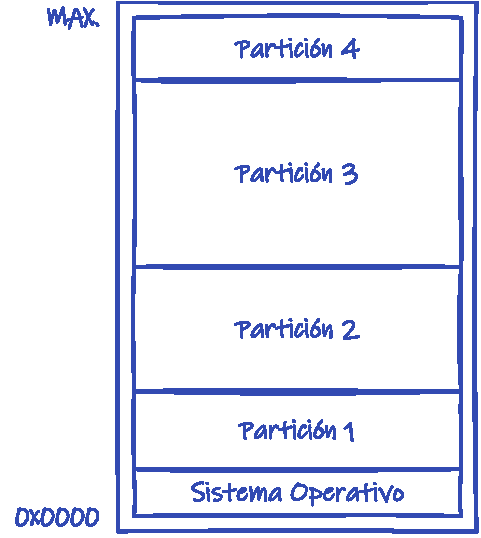
\includegraphics[width=0.8\textwidth]{media/C15_memoria_principal/particionado_fijo.pdf}
\caption{Particionado fijo de la memoria en el IBM OS/360.}
\end{figure}

Este método fue utilizado originalmente por el \{ibmos360\}, pero ya no
se utiliza

\subsection{Particionado dinámico}\label{_particionado_dinuxe1mico}

{} El \textbf{particionado dinámico} es una generalización del anterior:

\begin{enumerate}
\def\labelenumi{\arabic{enumi}.}
\item
  El sistema operativo mantiene una tabla indicando qué partes de la
  memoria están libres y cuáles ocupadas. Inicialmente toda la memoria
  está libre por lo que es considerada como un gran hueco de memoria
  disponible.
\item
  Cuando un proceso llega y necesita memoria, se le busca un hueco lo
  suficientemente grande para alojarlo. Si se encuentra, solo se le
  asigna el espacio necesario, que es marcado como ocupado. El resto
  sigue siendo un hueco libre, aunque de menor tamaño.
\item
  Si un proceso termina y se crean dos huecos adyacentes, se funden en
  uno solo.
\end{enumerate}

El \textbf{particionado dinámico} se utilizaba fundamentalmente en
\textbf{sistemas de procesamiento por lotes} y
\textbf{multiprogramados}. En este último caso, el sistema operativo
tenía una \textbf{cola de entrada} ordenada por el \textbf{planificador
de largo plazo} y la recorría asignando memoria a los procesos, hasta
que no quedara ningún hueco libre con tamaño suficiente para alojar al
siguiente en la cola. Entonces el sistema operativo podía esperar hasta
que algunos procesos terminarán y hubiera un hueco lo suficientemente
grande en la memoria, para el siguiente proceso, o podía seguir buscando
en la cola de entrada procesos de menores requerimientos, aunque para
ello tuviera que saltarse algunos procesos.

En general, en un momento dado el sistema operativo, debe satisfacer una
petición de tamaño \emph{N} con una lista de huecos libres de tamaño
variable. Esto no es más que un caso particular del problema clásico de
la asignación dinámica de almacenamiento, para el cual hay diversas
soluciones:

\begin{itemize}
\item
  En el \textbf{{}primer ajuste}{} se escoge el primer hueco lo
  suficientemente grande como para satisfacer la petición. La búsqueda
  puede ser desde el principio de la lista o desde donde ha terminado la
  búsqueda anterior.
\item
  En el \textbf{{}mejor ajuste}{} se escoge el hueco más pequeño que sea
  lo suficientemente grande para satisfacer la petición. Indudablemente
  esto obliga a recorrer la lista de huecos completa o a tenerla
  ordenada por tamaño.
\item
  En el \textbf{{}peor ajuste}{} se escoge el hueco más grande.
  Igualmente obliga a buscar en toda la lista de huecos o a tenerla
  ordenada por tamaño.
\end{itemize}

Para evaluar qué estrategia es la mejor, se han realizado algunas
simulaciones con los siguientes resultados:

\begin{itemize}
\item
  El \textbf{primer y el mejor ajuste} son mejores que el peor ajuste en
  términos de menor tiempo y mayor aprovechamiento del espacio de
  almacenamiento.
\item
  Si comparamos el \textbf{primer y el mejor ajuste} ninguno de ellos
  destaca sobre el otro en lo que a mejor aprovechamiento del espacio se
  refiere.
\item
  El \textbf{primer ajuste} es normalmente más rápido que el
  \textbf{mejor ajuste}.
\end{itemize}

\section{Fragmentación}\label{_fragmentaciuxf3n}

{} Las estrategias de asignación de espacio de almacenamiento
generalmente sufren de problemas de \textbf{fragmentación}. Vamos a
comentar brevemente cómo afecta la \textbf{fragmentación} a la
\textbf{asignación contigua de memoria}.

\subsection{Fragmentación externa}\label{_fragmentaciuxf3n_externa}

{} La \textbf{fragmentación externa} ocurre cuando hay suficiente
espacio libre para satisfacer una petición, pero el espacio no es
contiguo. Es decir, el espacio de almacenamiento está fraccionado en un
gran número de huecos de pequeño tamaño:

\begin{itemize}
\item
  Afecta tanto a la estrategia del \textbf{primer} como del
  \textbf{mejor ajuste}. Siendo el primero mejor en algunos sistemas y
  el segundo mejor en otros.
\item
  Algunos análisis estadísticos realizados con el \textbf{primer ajuste}
  revelan que incluso con algunas optimizaciones, con \emph{N} bloques
  asignados se pierden 0.5\emph{N} por \textbf{fragmentación externa}
  ---es decir, un tercio de toda la memoria no es utilizable---. A esto
  se lo conoce como la regla del 50\%.
\end{itemize}

Existen diversas soluciones a este problema:

\begin{itemize}
\item
  Utilizar técnicas de \textbf{{}compactación}, lo que consiste en mover
  los procesos para que toda la memoria libre quede en un único hueco de
  gran tamaño. Sin embargo, esto puede ser muy caro en términos de
  tiempo y solo puede ser realizado cuando la \textbf{asignación de
  direcciones absolutas se realiza en tiempo de ejecución}.
\item
  La otra solución es permitir que el \textbf{espacio de direcciones
  físico} de un proceso no sea contiguo. Es decir, que la memoria puede
  ser asignada a un proceso independientemente de donde esté disponible.
  Existen dos técnicas complementarias que utilizan esta solución: la
  paginación (véase el \hyperref[paginaciuxf3n]{???}) y la
  \href{https://es.wikipedia.org/wiki/Segmentaci\%C3\%B3n_de_memoria}{segmentación}.
\end{itemize}

\subsection{Fragmentación interna}\label{_fragmentaciuxf3n_interna}

{} La \textbf{fragmentación interna} se origina por la diferencia entre
el espacio solicitado y el espacio finalmente asignado.

Supongamos un hueco de espacio libre de 12987 bytes que se va a usar
para satisfacer una petición de 12985 bytes. Esto genera un hueco de 2
bytes, pero la cantidad de información que debemos guardar en la lista
de huecos para saber que dicho hueco está ahí, es mucho mayor que el
tamaño del hueco en sí mismo. Por lo tanto, no nos interesa tener huecos
de tamaño arbitrario.

La solución más común es dividir la memoria física en unidades de tamaño
fijo y asignarla en múltiplos del tamaño de dichos bloques. Esto hace
que, en general, se asigne más memoria de la que realmente se ha
solicitado y, por tanto, de la que realmente los procesos van a
utilizar. A esto se lo denomina \textbf{fragmentación interna}.

\section{Intercambio}\label{_intercambio}

{} {} Un proceso debe estar en la memoria para ser ejecutado, pero en
algunos sistemas operativos un proceso puede ser sacado de la memoria y
copiado a un almacenamiento de respaldo de forma temporal
---generalmente un dispositivo de almacenamiento secundario, como un
disco--- y en algún momento volver a ser traído a la memoria para
continuar su ejecución. Al procedimiento descrito se lo denomina
\textbf{intercambio} o \textbf{\emph{swapping}}.

\subsection{Implementación}\label{_implementaciuxf3n}

El \textbf{intercambio} se puede implementar de la siguiente manera:

\begin{enumerate}
\def\labelenumi{\arabic{enumi}.}
\item
  La \textbf{cola de preparados} contiene todos los procesos que esperan
  para ser ejecutados en la CPU.
\item
  Cuando el \textbf{planificador de la CPU} decide ejecutar un proceso,
  llama al \textbf{asignador}.
\item
  El \textbf{asignador} comprueba si el siguiente proceso que debe ser
  ejecutado está en la memoria. Si no lo está y no hay memoria libre, el
  \textbf{asignador} hace que el \textbf{gestor de la memoria}
  intercambie el proceso con alguno de los que sí lo está.
\item
  Finalmente, el \textbf{asignador} ejecuta el resto del cambio de
  contexto (véase el \hyperref[_cambio_de_contexto]{???}) para entregar
  la CPU al proceso seleccionado.
\end{enumerate}

Por ejemplo, si a un sistema con \textbf{planificación de CPU} basado en
prioridad llega a la \textbf{cola de preparados} un proceso de alta
prioridad, el \textbf{gestor de memoria} intercambia algunos procesos de
baja prioridad con el de alta prioridad y ejecuta este último. Cuando el
proceso de alta prioridad termina, los de baja prioridad pueden ser
intercambiados para continuar su ejecución.

\subsection{Limitaciones}\label{_limitaciones}

Sin embargo el \textbf{intercambio} presenta algunas limitaciones
importantes:

\begin{itemize}
\item
  Si un sistema \textbf{reubica las direcciones en tiempo de compilación
  o carga}, el proceso solo puede ser intercambiado en la misma región
  de la memoria. Sin embargo, si se utiliza \textbf{reubicación en
  tiempo de ejecución}, entonces el proceso puede ser intercambiado en
  cualquier región de la memoria, puesto que las \textbf{direcciones
  físicas} son calculadas durante la ejecución.
\item
  El \textbf{tiempo de cambio de contexto} en un sistema con
  \textbf{intercambio} puede ser mucho mayor, puesto que incluye el
  tiempo que se tarda en hacer el intercambio. La mayor parte del tiempo
  de intercambio es el tiempo de transferencia con el disco, que puede
  ser de varios cientos de milisegundos, incluso utilizando los discos
  más rápidos. Esto afecta al \textbf{tiempo de cuanto} que siempre debe
  ser mucho mayor que el tiempo de \textbf{cambio de contexto}.
\item
  Un proceso podría disponer de un espacio en memoria de 120 MiB pero
  estar utilizando solo 2 MiB. Por tanto, es interesante que el sistema
  operativo conozca con exactitud la memoria utilizada por el proceso
  ---y no la que podría estar utilizando como máximo--- para reducir el
  tiempo de transferencia de los datos al disco durante el intercambio.

  Para eso, el sistema operativo proporciona llamadas al sistema con las
  que un proceso con requerimientos dinámicos de memoria puede informar
  del cambio en su necesidad de memoria. Por ejemplo, los sistemas
  operativos modernos proporcionan llamadas al sistema para reservar y
  liberar memoria ---como \{clang\_malloc\} y \{clang\_free\} en los
  sistemas POSIX--- gracias a las que el sistema conoce las necesidades
  reales de los procesos.
\item
  El \textbf{intercambio} presenta dificultades cuando el proceso que va
  a ser sacado de la memoria está esperando por una operación de E/S que
  accede a la memoria del proceso para leer o escribir datos en ella.
  Las soluciones podrían ser:

  \begin{itemize}
  \item
    No intercambiar procesos con operaciones de E/S síncronas o
    asíncronas pendientes.
  \item
    Utilizar búferes del sistema operativo en las operaciones de E/S.
    Por ejemplo, en una operación \textbf{write} a un archivo, el
    sistema operativo copiaría primero los datos a un búfer interno y
    luego ordenaría la escritura de esos datos. Así el proceso podría
    ser intercambiado sin problemas. Las transferencias entre los
    búferes del sistema y la memoria de los procesos serían realizadas,
    por el sistema operativo, solo cuando los procesos residen en la
    memoria.
  \end{itemize}
\end{itemize}

Debido fundamentalmente a que el tiempo de intercambio es muy alto, no
se utiliza el intercambio estándar en los sistemas operativos actuales.
Lo que sí podemos encontrar en muchos sistemas son versiones modificadas
de este mecanismo.

Por ejemplo, en muchas versiones antiguas de UNIX y en los sistemas
modernos, el intercambio permanece desactivado y solo se activa cuando
la cantidad de memoria usada supera cierto límite. Además, en los
sistemas actuales no se intercambian procesos completos si no las
porciones menos usadas de cada proceso, como veremos en el
\hyperref[memoria_virtual]{???}.
